\newpage
\section{Thermal cycling of detector's electronics}
\label{thermal_cycling}

The Front-End Electronics of the \gls{STS} will undergo significant thermally induced mechanical stresses over the detector's lifetime. During the commissioning and configuration, the \gls{FEE}, especially the \glspl{FEB} will undergo many power cycles. As reported in the~\cite{CBM_PR_2021}, the power cycling of the \glspl{FEB} in room temperature of about \SI{20}{\celsius} run flawlessly, not identifying any issues with the \glspl{FEB}. Nevertheless, the testing did not reproduce the conditions that we will face during the \gls{STS} operation.

Operating scenarios of the \gls{STS} together with other constraints related to, for example, the soft errors rate in the low voltage powering of the \gls{FEE}, define the testing procedures for all the electronics which will face mechanical stresses. For the control and monitoring of the devices, as well as for processing of the data the previously developed control framework was introduced. 
\subsection{Nominal operation scenario of STS}
\label{nominal}

Cooling liquid at \SI{-40}{\celsius}, \gls{FEB}s powered on.
    As per the simulations done for the cooling liquid entering the detector at  \SI{-40}{\celsius}, the cooling plate and \gls{FEB}s should reach temperatures as shown in Figure~\ref{fig_coolinkg_block_nominal} and~\ref{fig_nominal_febs}.

    
\begin{figure}[!h]
\centering
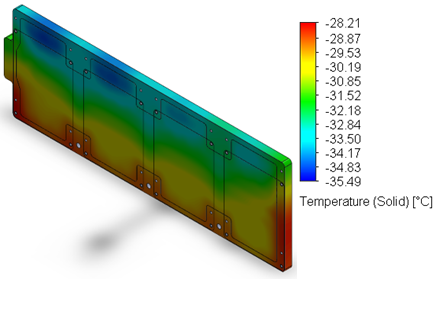
\includegraphics[width=0.6\columnwidth]{Chapter4/images/cooling_block_nominal.png}
\caption{Temperature distribution on the cooling plate for the nominal operation scenario~\cite{thermal_cycling}.}
\label{fig_coolinkg_block_nominal}
\end{figure}

\begin{figure}[!h]
\centering
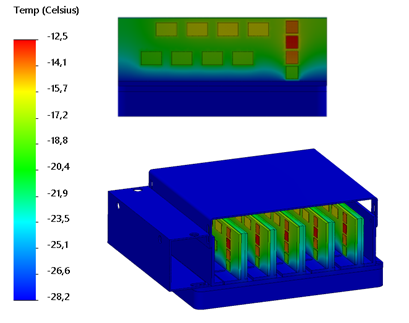
\includegraphics[width=0.5\columnwidth]{Chapter4/images/nominal_febs.png}
\caption{Temperature distribution in the \gls{FEB} box and in the \gls{FEB} for the nominal operation scenario~\cite{thermal_cycling}.}
\label{fig_nominal_febs}
\end{figure}


In periods in which the temperature will change due to transitions between detector states. The electronics will also face thermal stresses, which will partially occur with the electronics switched on. During the active (with low voltage on) phase of operation, the temperature change of the electronics could be $\Delta T \approx \SI{20}{\celsius}$. After switching off the electronics, the temperature change is $\Delta T \approx \SI{20}{\celsius}$. These temperatures provide an indication of minimum and maximum thermal cycling set points.  
%\begin{figure}[!h]
%\centering
%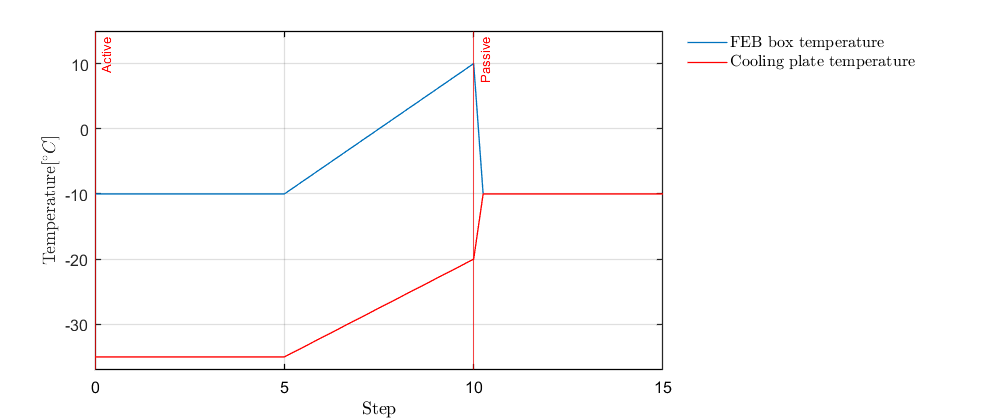
\includegraphics[width=0.95\columnwidth]{Chapter4/images/nominal_all.png}
%\caption{An example of \gls{STS} state transition from operation to safe state - comparison of temperatures of a %\gls{FEB} box and cooling liquid temperature.}
%\label{fig_nominal_scenario}
%\end{figure}
%\newpage

\subsection{Reboot scenario of STS}
\label{reboot}

At any given point during operation, the operator may need to reconfigure or reboot a \gls{FEB}(s). In this scenario, the temperature of a given \gls{FEB} may change dramatically due to a temporary lack of power. How much thermally induced mechanical stress the \gls{FEB} will face depends on reboot and configuration time. In case of a radiation-induced soft error in the power supply, the downtime of a \gls{FEB} may be difficult to predict. 

The simulations below were prepared for a case in which the passive \gls{FEB} reach the equilibrium temperature. Figure~\ref{fig_reboot_box} depicts the scenario in which only 5 out of 10 \glspl{FEB} are on, which results in effectively lower temperatures in comparison to the nominal scenario. Nevertheless, the $\Delta T$ remains the same as in the nominal operation scenario. In reality, the reboot scenario will probably last for a short time (range of seconds) and the temperature of the rebooted \gls{FEB} will not reach as low temperatures as depicted in the previous simulations.


%\begin{figure}[!h]
%\centering
%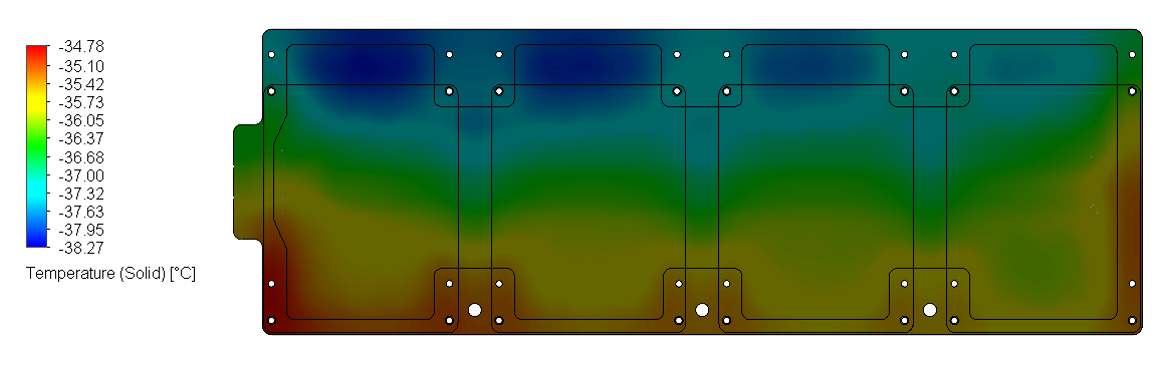
\includegraphics[width=0.85\columnwidth]{Chapter4/images/reboot_cooling_plate.png}
%\caption{Temperature distribution on the cooling plate for the reboot scenario}
%\label{fig_reboot_scenario}
%\end{figure}

\begin{figure}[!h]
\centering
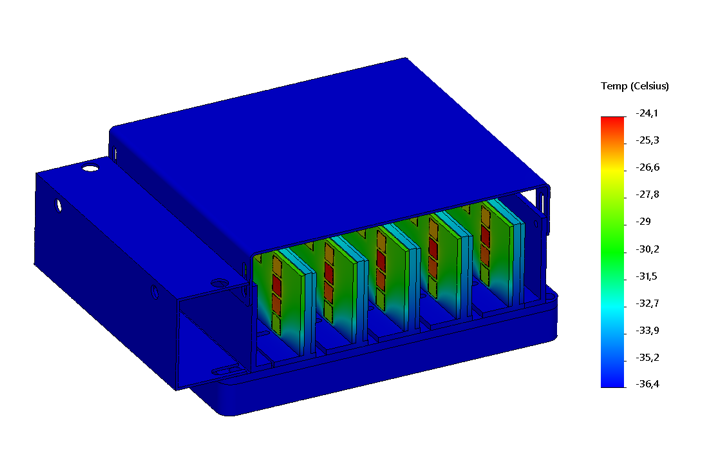
\includegraphics[width=0.6\columnwidth]{Chapter4/images/reboot_box.png}
\caption{Temperature distribution in the \gls{FEB} box for the reboot scenario~\cite{thermal_cycling}.}
\label{fig_reboot_box}
\end{figure}

\begin{figure}[!h]
\centering
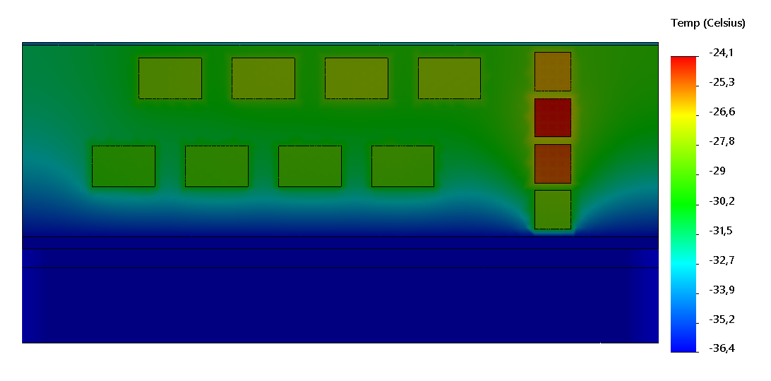
\includegraphics[width=0.6\columnwidth]{Chapter4/images/reboot_FEB.png}
\caption{An example of \gls{STS} state transition from operation to safe state - comparison of temperatures of a \gls{FEB} box and cooling liquid temperature~\cite{thermal_cycling}.}
\label{fig_reboot_FEB}
\end{figure}

%\begin{figure}[!h]
%\centering
%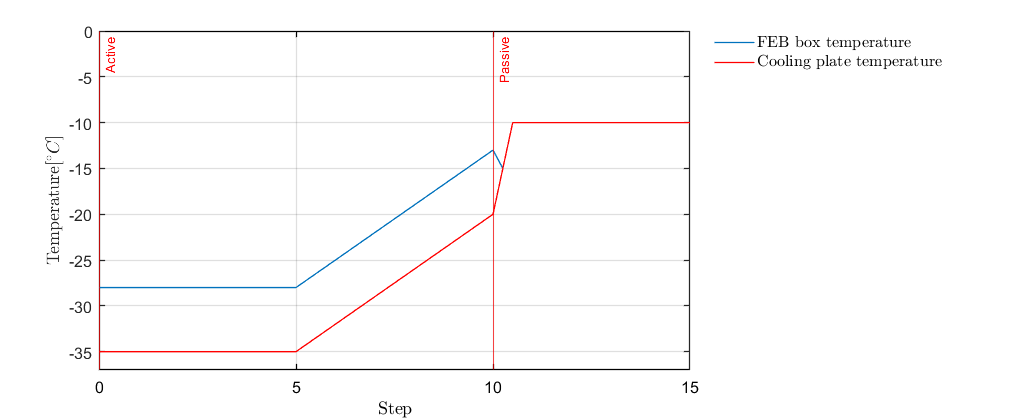
\includegraphics[width=0.95\columnwidth]{Chapter4/images/nominal.png}
%\caption{An example of \gls{STS} state transition from operation to safe state - comparison of temperatures of a %\gls{FEB} box and cooling liquid temperature.}
%\label{fig_reboot_nominal}
%\end{figure}
%\newpage
\subsection{Loss of power scenario of STS}
\label{power_loss}
The last considered scenario is the so-called loss of power scenario. Out of the three introduced scenarios, it's the least probable one, but it also leads to a significant data loss, as 10 \glspl{FEB} would stop sending data. Such a scenario could happen if all the connected low-voltage channels switch off, e.g. due to radiation. In this case, the \glspl{FEB} would reach the temperature of the cooling block ($T \approx \SI{-40}{\celsius}$) if the powering wasn't turned in a timely manner.
Thermal cycling testing is usually performed in order to determine the ability of different components and solder interconnects to resist extreme temperature changes. Permanent changes to the electrical or physical features may compromise the detector modules' performance. 
\subsection{Thermal cycling and potential consequences for the Front-End Board}

The thermal expansion coefficient (\gls{CTE}) is an important property of adhesives that affects relative movement between parts on a \gls{PCB}. \gls{CTE} should be a concern when it comes to \glspl{PCB}, as out-of-plane \gls{CTE} could cause cracking and delamination, while in-plane \gls{CTE} may for example cause shear failures in solder joints~\cite{cte_report}. In the case of the \glspl{FEB} both the \gls{LDO} regulators and STS-XYTERs are glob-topped, therefore identifying potential reasons for failure could be a complex task. Apart from \gls{CTE}, the performance of a \footnote{protective epoxy-based material for microelectronics}{glob top} material depends on many other factors:
\begin{itemize}
    \item adhesion to the substrates,
    \item part geometry (including mass),
    \item temperature extremes,
    \item cycle and transition times.
\end{itemize}
DYMAX 9001 was the glob top choice for the \glspl{FEB}, and it was then replaced by its successor DYMAX 9014. In this case, to simplify the problem, we assume that \gls{LDO} regulators and \glspl{ASIC} are mainly composed of silicon. The linear CTE of glob top materials (DYMAX 9001, DYMAX 9014, DYMAX 9008) and conductive glue (EPO-TEK E4110) is one order of magnitude higher than the coefficient for the \glspl{PCB} and silicon. Additionally, a volume expansion should be considered to understand the overall situation.

From the thermal cycling point of view, the most significant difference between the DC linear voltage regulator and the front-end chip is the power dissipation. The \gls{LDO} regulator dissipates much more heat than the STS-XYTER (see photo~\ref{fig_temperatures_camera}), which was also confirmed by multiple simulations (see sections~\ref{nominal} -~\ref{power_loss}).

\begin{figure}[!h]
\centering
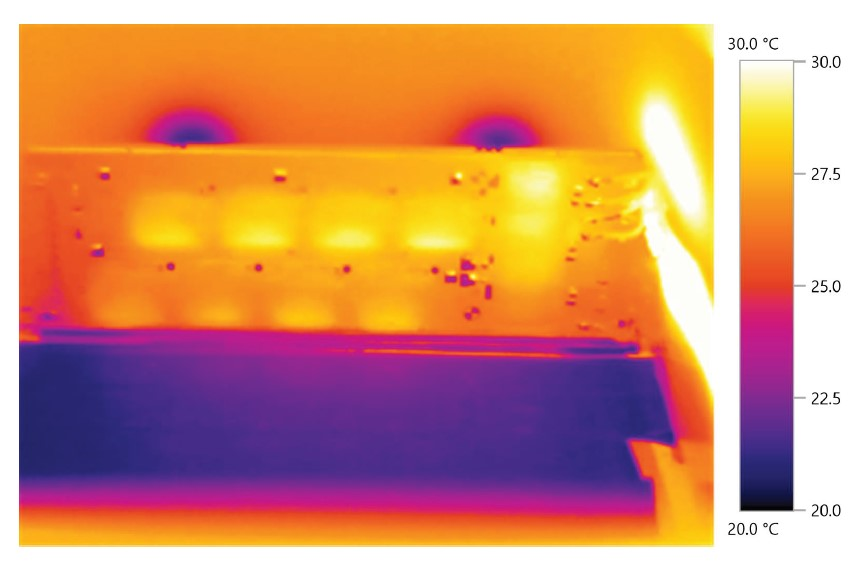
\includegraphics[width=0.6\columnwidth]{Chapter4/images/feb_thermal.jpg}
\caption{Temperature of the \gls{FEB} components measured with a thermal camera for the low power consumption scenario, \cite{leo_electronics}. The \gls{LDO} (on the right side of the photo) dissipates on average more heat than chips.}
\label{fig_temperatures_camera}
\end{figure}


\begin{table}[!h]
\begin{center}
\caption{Coefficient of thermal expansion of different materials below the glass transition temperature.}
\begin{tabular}{ll}
\hline
\multicolumn{1}{c}{Material} & \multicolumn{1}{c}{CTE $\alpha_{2}$} [\si{\micro\metre\per\metre\per\celsius]}] \\ \hline
DYMAX 9001-E-V3.5~\cite{9001}            & 180                                  \\
DYMAX 9014~\cite{9014}                   & 192                                  \\
EPO-TEK E4110~\cite{4110}                & 150                                  \\ \hline
FR4~\cite{FR4}                          & 15                                   \\
Si~\cite{Si}                           & 2.6                                 
\end{tabular}
\label{TCE}
\end{center}
\end{table}

\newpage
%\newpage


There are other phenomena that may cause damage to a glob-topped device:
\begin{itemize}
    \item chip cracking,
    \item failure of the chip to board or substrate joint,
    \item damage to protective chip passivisation layer,
    \item wire-bond failure,
    \item metallization pattern shift,
    \item development of voids or notches in metallization tracks. 
\end{itemize}


According to the data analyzed by the U.S. Air Force over about 20 years, it was shown that 50\% of these failures are related to connectors, 30\% to interconnects, and 20\% to component
parts. Hardware failures may occur due to handling, vibrations, or stress of different origins (including thermal stress). About 55\% of the electronics failures are due to high temperatures and temperature cycling, 20\% of the failures are related to vibration and shock, and 20\% are due to humidity~\cite{thermal_electronics}. 



%\begin{figure}[!h]
%\centering
%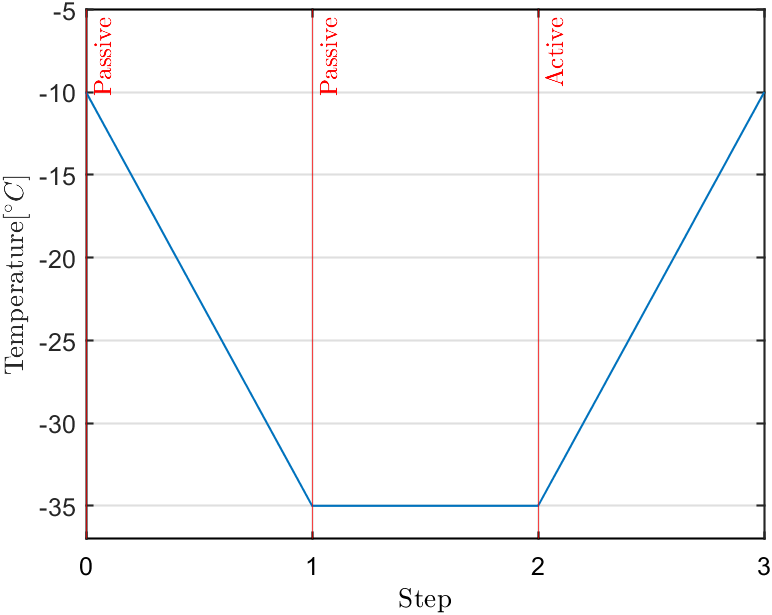
\includegraphics[width=0.55\columnwidth]{Chapter4/images/switchoff.png}
%\caption{Sudden loss of power and bringing the \glspl{FEB} back to operation}
%\label{fig_loss}
%\end{figure}

%\newpage
\subsection{Experimental setup for thermal cycling of STS electronics}
\label{cycling_setup}
The experimental setup for the thermal cycling is depicted in Figure~\ref{fig_setup}. The software part features the Control System Studio (Phoebus) for monitoring, accessing the database (Redis DB), and monitoring the \gls{PV}s. Moreover, all values are saved with archiver appliance. The second node dedicated to thermal cycling features a LabView-based interface for reading out additional humidity sensors. This node was later on depreciated and relative humidity readouts were taken from the built-in Relative Humidity (\gls{RH}) sensor inside the climatic chamber.

The main test object for this part of the work was thermal cycling of the \gls{FEB}s. The diagnostic circuit of the STS-XYTER helps to identify any \gls{PCB} related issues. In order to read the temperatures, VDDM, and  \gls{CSA} bias values, a dedicated \footnote{purely software-based \gls{IOC}, not connected to any hardware}{soft IOC} was deployed. To acquire the previously mentioned values, the pyEPICS library~\cite{pyEPICS} was used, and the GBTxEMU-based readout chain (see \autoref{tester}) was adjusted to publish the values via channel access protocol. 
\begin{figure}[!h]
\centering
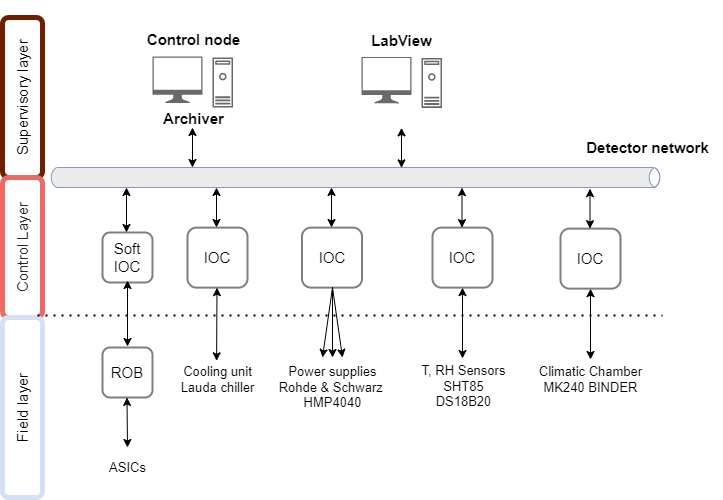
\includegraphics[width=0.85\columnwidth]{Chapter4/images/cycling_scheme.png}
\caption{Schematics of the thermal cycling setup. The readout of relative humidity and temperature sensor is realized through Single Board Microcontrollers~(\gls{SBC}) and Raspberry PI.}
\label{fig_setup}
\end{figure}
Apart from the \gls{ASIC}-specific values, we monitor also:
\begin{itemize}
    \item currents and voltages supplied to the 1.2V and 1.8V \gls{LDO} regulators on the \gls{FEB}, 
    \item temperature changes on the fin (as seen in Figure~\ref{fig_cycling_temps}), which are read-out by a Single Board Microcontroller \gls{SBM},
    \item humidity and temperature in the climatic chamber (Sensiron SHT85 sensors plus built-in sensors),
    \item set point temperature of the Kryo 51 coolant~\cite{KRYO}.
\end{itemize}

The \gls{FEB}s components may slightly differ, depending on what was the aim of the cycling for a given \glspl{PCB}. We can distinguish three board flavors:
\begin{itemize}
    \item with DYMAX 9001 as the glob top (see photo~\ref{fig_noglobtop}),
    \item with DYMAX 9001 as the fill and DYMAX 9008 as the dam (see photo~\ref{fig_cycling_temps}), 
    \item without glob top and \glspl{ASIC} (see photo~\ref{fig_noglobtop}).
    \end{itemize}
\newpage
\begin{figure}[!h]
\centering
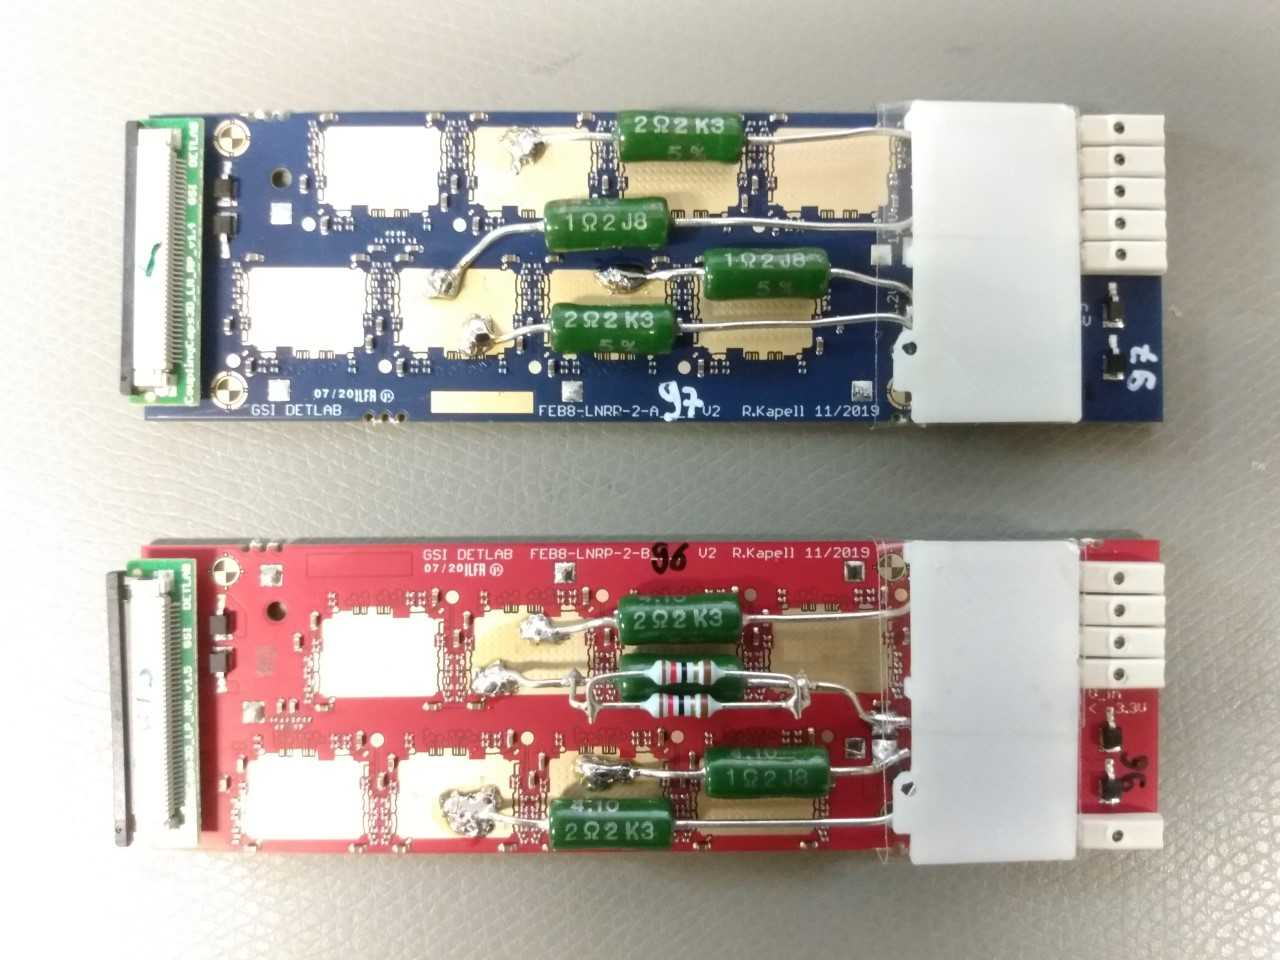
\includegraphics[width=0.45\columnwidth]{Chapter4/images/noglobtop.jpg}
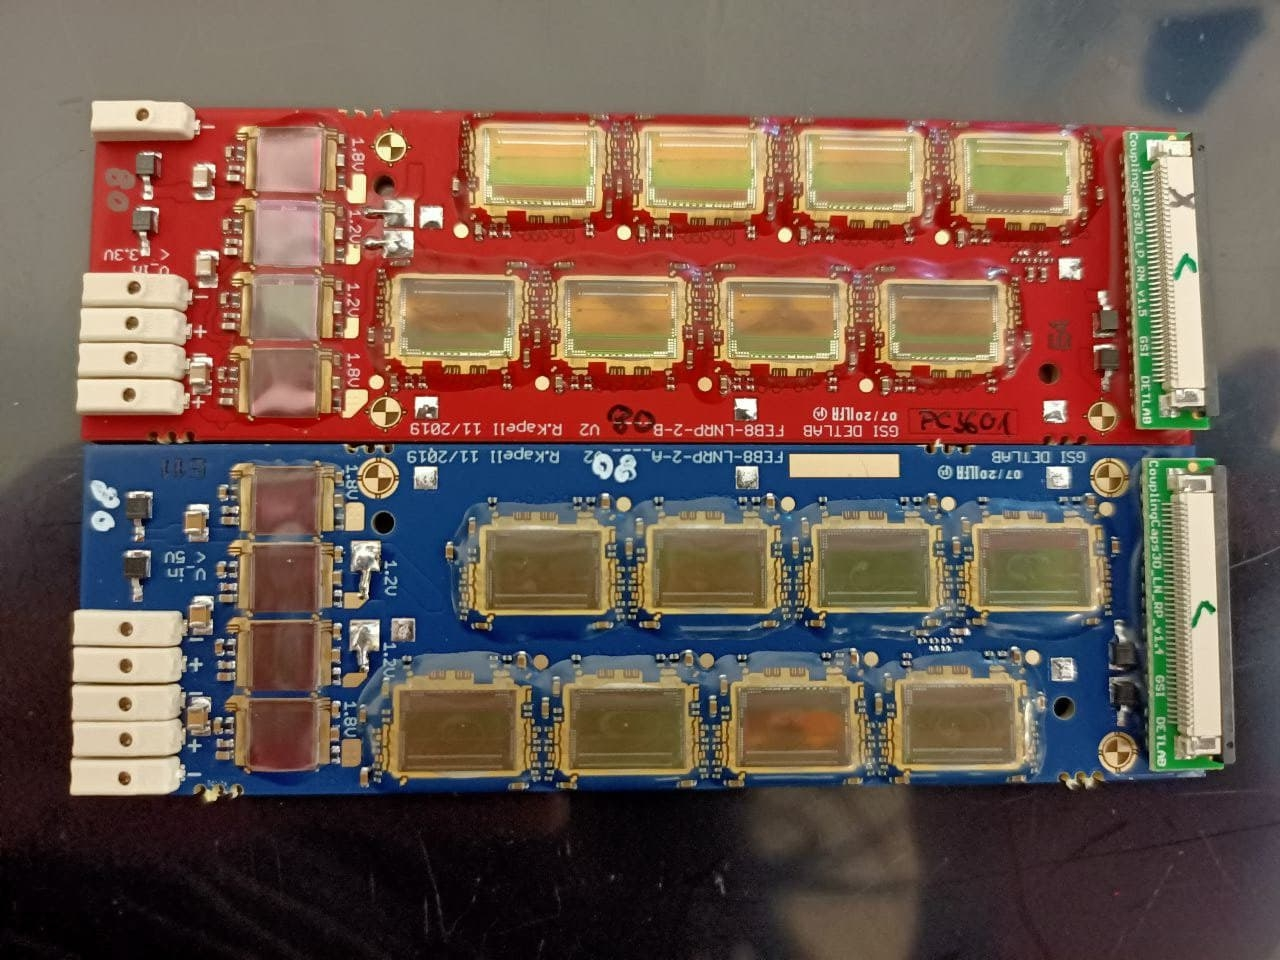
\includegraphics[width=0.45\columnwidth]{Chapter4/images/globtop.jpg}
\caption{Left photo depicts two \glspl{FEB} (version A and B) with the \gls{LDO} regulators with a 3D-printed protection cover and without glob top. These two boards feature also have resistors simulating the power consumption of the STS-XYTERs.
The right photo depicts two fully assembled \gls{FEB}s with STS-XYTERS version 2.1 and DYMAX 9001 as the glob top.}
\label{fig_noglobtop}
\end{figure}

To prepare for the thermal cycling, the assembled boards (type A and B) were mounted on a cooling fin (either with thermal pads or by gluing it to the fin's surface) and then subsequently placed on a cooling plate in the climatic chamber (see Figure~\ref{fig_cycling_temps}). In order to reproduce similar conditions as in the \gls{STS} (coolant temperature at \SI{-40}{\celsius}) KRYO 51 coolant instead of the NOVEC 649. Additionally, the temperature of the chamber is always kept below the temperature of the cooling plate to avoid icing. During the cycling, the voltage drop at the \gls{LDO} regulators was the same for all the boards \SI{0.6}{\volt}.

\begin{figure}[!h]
\centering
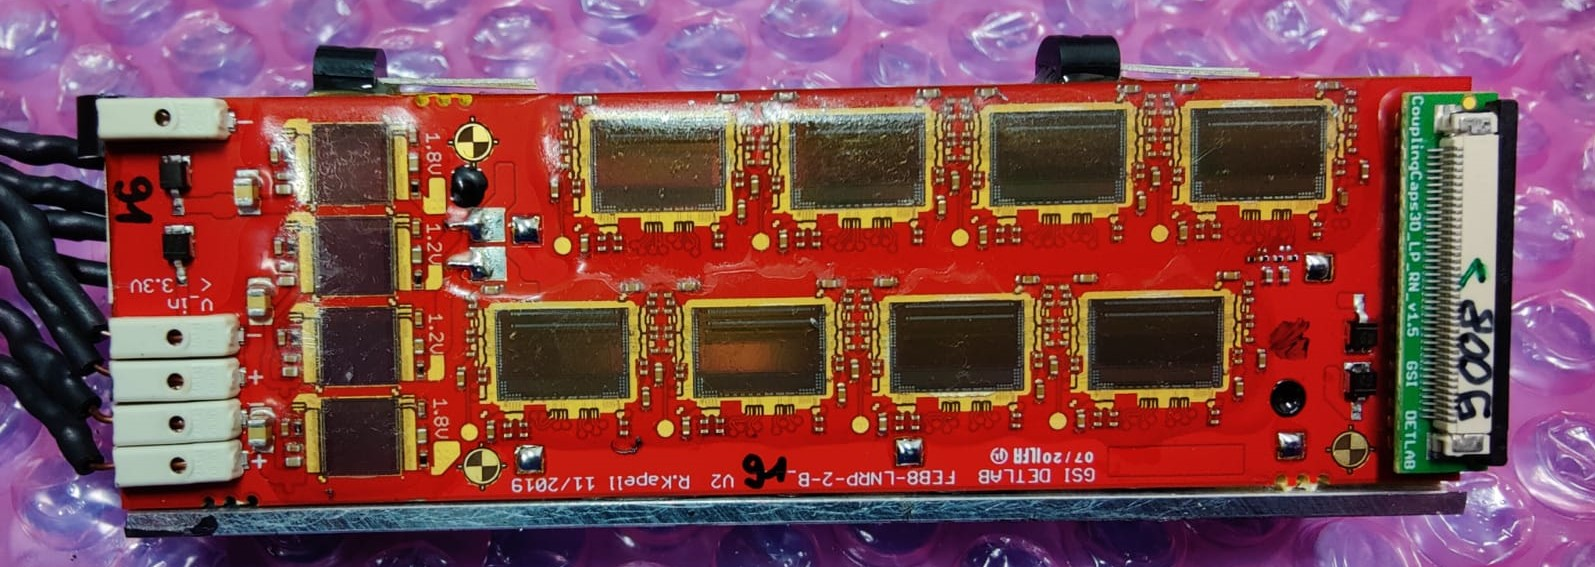
\includegraphics[width=0.5\columnwidth]{Chapter4/images/FEBB_T_sensors.jpeg}
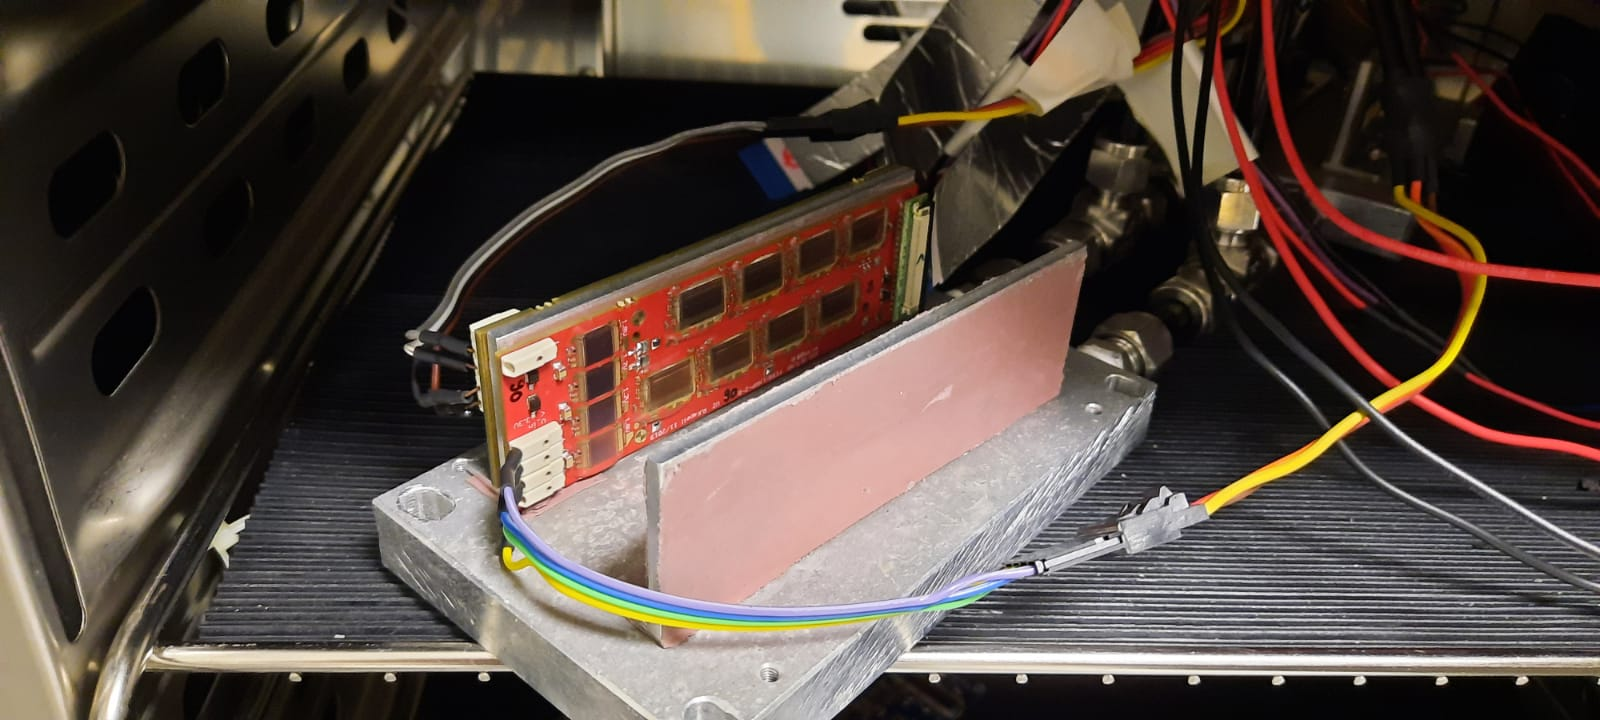
\includegraphics[width=0.4\columnwidth]{Chapter4/images/thermal_setup.jpeg}
\caption{A \gls{FEB} glued to the fin, with 3 DS18B20 temperature sensors installed on the fin (left) and two \gls{FEB}s mounted on a fin with thermal pads inside a climatic chamber (right).}
\label{fig_cycling_temps}
\end{figure}

\newpage

\subsection{Testing procedure}
Based on the operation scenarios of the \gls{STS}, the \gls{FEB}s, \gls{ROB}s, and \gls{POB}s need to withstand:
\begin{itemize}
    \item without the powering - $\Delta T\approx\SI{20}{\celsius} $
    \item with powering - $\Delta T\approx\SI{20}{\celsius} $
    \item more than 190 cold startups, as indicated in section~\ref{irradiation_results}
\end{itemize}
Testing was divided into three stages: passive cycling, active cycling, and power cycles down to \SI{-40}{\celsius} (so-called cold startup). The transition time between the extreme temperatures (for passive and active cycling) was not manually adjusted and depends only on the power of the Lauda chiller and the climatic chamber. 

The main object of the tests was the \gls{FEB}s and its sensitivity to the thermally induced mechanical stresses. In the two main sets of measurements so far, in total 12 \gls{FEB}s in different configurations were tested.  After each round of thermal cycling, the boards were inspected optically under the microscope for any signs of deterioration or visible changes. On the other hand, during the cycling with powering and cold startups, the STS-XYTERs were extensively tested. The \glspl{ASIC} test included configuration of the chip, changing \gls{CSA} values to trigger different current consumption, but also ID consistency check, write/read registers test, and internal pulses. 
\subsubsection{Passive cycling}

Passive cycling was performed in the series of 50 repetitions between optical and electrical inspection. During this part we tested the following temperature differences:
\begin{itemize}
    \item Set A - 8 \glspl{FEB} (3 \glspl{FEB} type A, 3 \glspl{FEB} type B and 2 \glspl{FEB} without glob top and \glspl{ASIC}) were tested in the realistic operating scenarios of the \gls{STS} - [\SI{-20}{\celsius}, \SI{-10}{\celsius}], [\SI{-30}{\celsius}, \SI{-10}{\celsius}], [\SI{-40}{\celsius}, \SI{-10}{\celsius}],
    \item Set B - 2/4 \glspl{FEB} (1/2 \glspl{FEB} A and 1/2 \glspl{FEB} B) were tested more extensively by increasing $\Delta T$ - [\SI{-20}{\celsius}, \SI{20}{\celsius}].
\end{itemize}
The \gls{FEB}, regardless of the type (A or B), are treated equally from the mechanical point of view. The components and the way the board is assembled are the same. Thereafter, the type won't be distinguished. During set B testing, there weren't any current trip conditions applied and for set A the trip current was set to 3.1 A. 
%The passive cycling is illustrated in Figure~\ref{fig_passive_cycling}.
The liquid pumped through the cooling block is always a few degrees higher (depicted as 'Lauda temperature') than the setpoint of the climatic chamber. This prevails condensation or icing on sensitive electronics at all times. The periods at the maximum and minimum temperature were always the same and equaled 20 minutes. During passive cyclings we haven't observed any performance deterioration, but it was always performed on brand-new boards.
%\begin{figure}[!h]
%\centering
%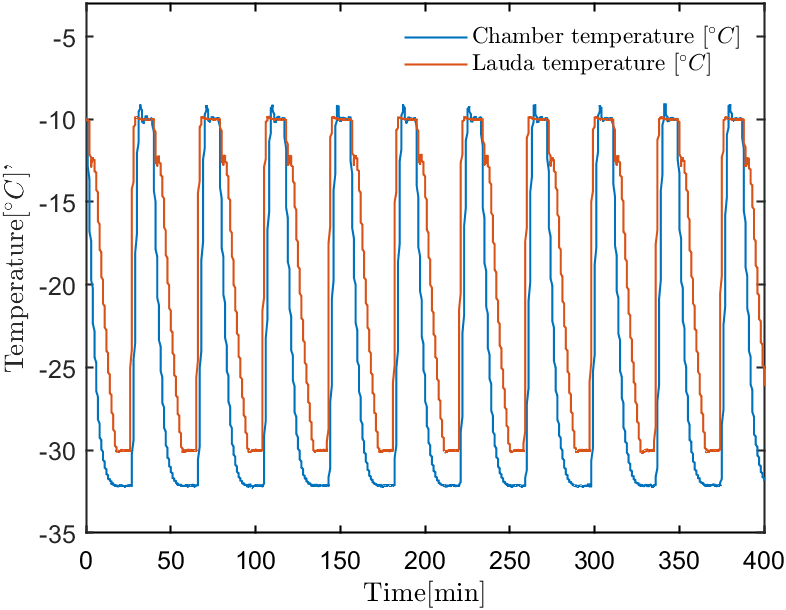
\includegraphics[width=0.55\columnwidth]{Chapter4/images/active_cycling.png}
%\caption{Example of the thermal cycling (passive) of the FEE}
%\label{fig_passive_cycling}
%\end{figure}

\subsubsection{Active cycling}
The active cycling was performed also in series of 50 repetitions, but due to the fact that the \glspl{FEB} were powered, all the boards and STS-XYTERs were continuously tested, and the current consumed varied by around 1 A at most. The boards underwent the followings cycles:
\begin{itemize}
    \item set A - 8 \glspl{FEB} - [\SI{-10}{\celsius}, \SI{20}{\celsius}] and [\SI{-40}{\celsius}, \SI{-10}{\celsius}],
    \item Set B - 4 \glspl{FEB} (2 \glspl{FEB} A and 2 \glspl{FEB} B)  $\Delta T$ - [\SI{-20}{\celsius}, \SI{20}{\celsius}], [\SI{-30}{\celsius}, \SI{20}{\celsius}], [\SI{-40}{\celsius}, \SI{20}{\celsius}].
\end{itemize}
A detailed view of a few cycles is presented in Figure~\ref{fig_active_detailed}. Figure depicts active cycling from \SI{-30}{\celsius} to \SI{20}{\celsius}.
\begin{figure}[!h]
\centering
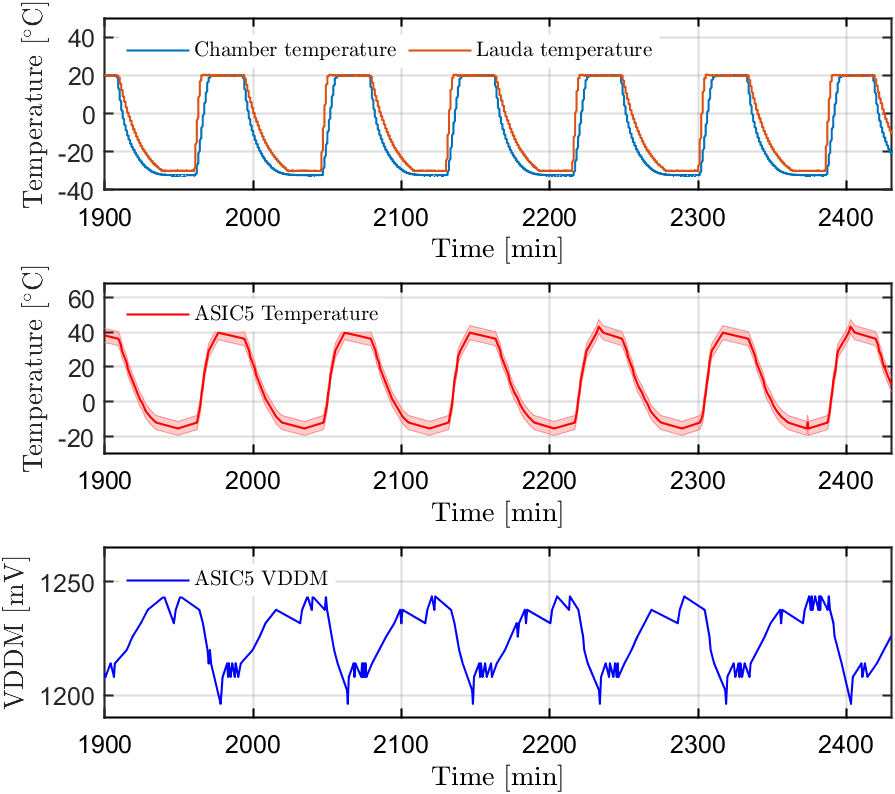
\includegraphics[width=0.65\columnwidth]{Chapter4/images/FEB0ASIC5COMP.png}
\caption{A detailed view on the performed active cycling. The top figure depicts the temperature of the chamber temperature and the set point of the Lauda chiller. Two lower figures show how the readout of temperature and VDDM from a chosen STS-XYTER depend on the cycling temperature. }
\label{fig_active_detailed}
\end{figure}

Similarly to passive cycling, the temperature of the cooling block is kept slightly above the ambient temperature, although the effective temperature of the active components (STS-XYTERs and \gls{LDO} regulators) is much higher. The two bottom plots show how the cycling affects the STS-XYTERs diagnostic circuit. The VDDM value varies from about 1200~mV up to 1240~mV, but it does not have any effect on the performance of the chip, as the operating range could vary as much as 100~mV. The measured values of the VDDM may also vary across the \gls{FEB}, which can be seen in Figure~\ref{feb_vary}. These differences highlight the need to properly calibrate the ADC of the diagnostic circuit, as the measured value shouldn't be too far from \footnote{considering that the voltage drop across the 1.2~V line connecting the subsequent chips is negligible}{the nominal 1.2~V} supplied by the 1.2~V \gls{LDO} regulator. 
\begin{figure}[!h]
\centering
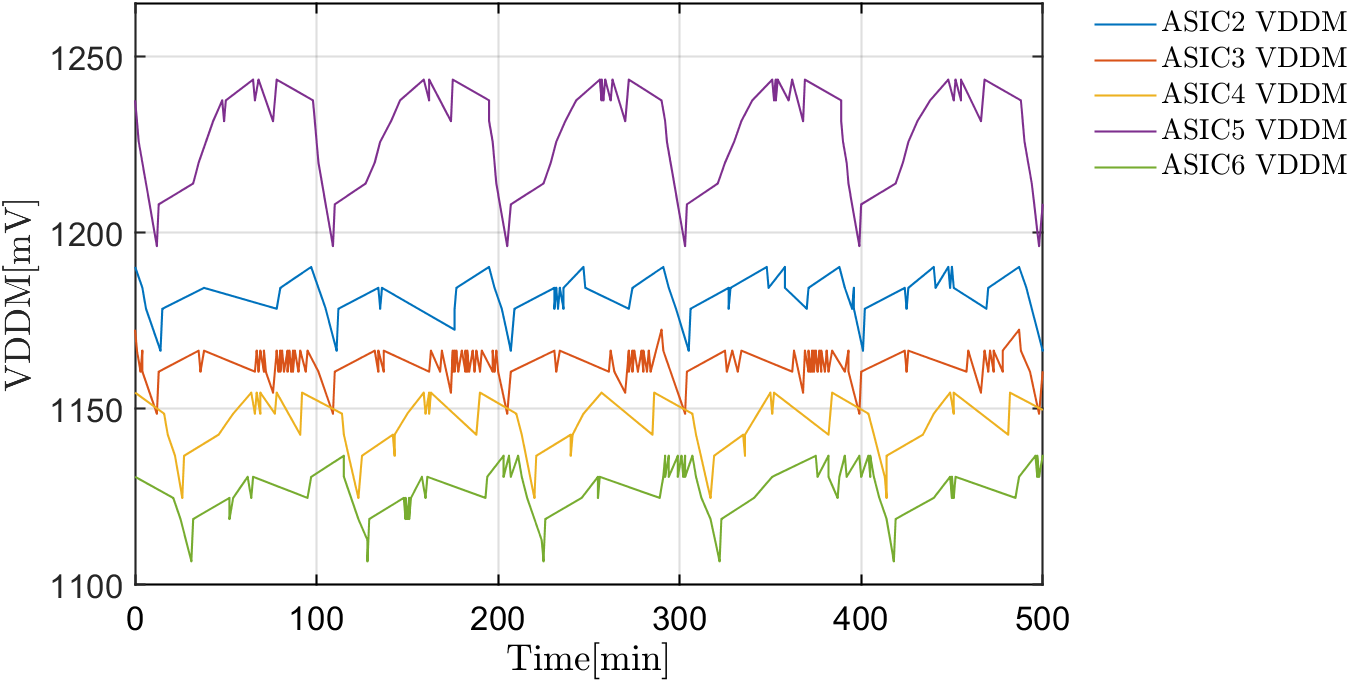
\includegraphics[width=0.9\columnwidth]{Chapter4/images/vddm_comp.png}
\caption{VDDM values comparison for different chips in the board.}
\label{feb_vary}
\end{figure}

%\newpage
Moreover, during the active cycling, we placed 3 DS18B20 sensors on the fin (see section~\ref{cycling_setup}. The sensors were glued to the fin, in order to determine how the temperature changes when the final thermal interfaces are used. Figure~\ref{fig_active_sensors} depicts the difference between the temperatures measured by different sensors during cycling. 

\begin{figure}[!h]
\centering
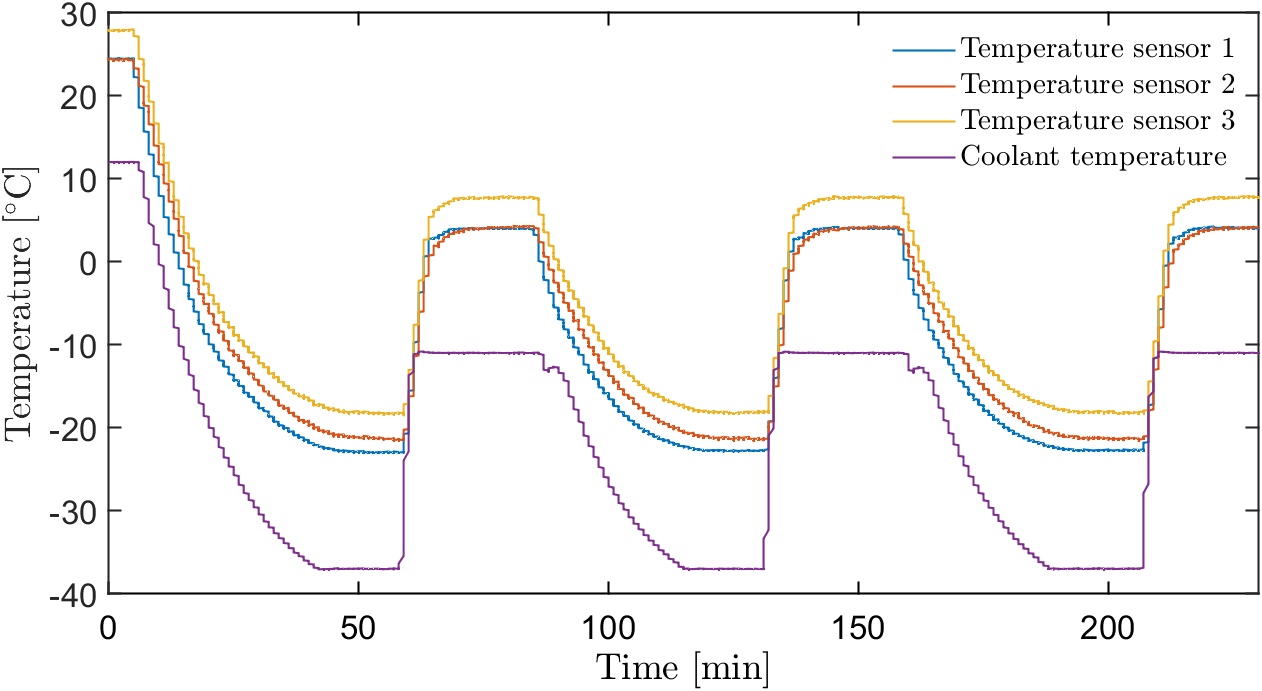
\includegraphics[width=0.5\columnwidth]{Chapter4/images/active.png}
\caption{Temperature evolution of the fin during the active cycling. The DS18B20 \cite{DS18B20} sensor has an uncertainty of $\SI{0.5}{\celsius}$.}
\label{fig_active_sensors}
\end{figure}


Temperature sensor 1 was placed above the \gls{LDO} regulators, therefore the measured values are always higher than for the two other sensors. Temperature sensor 2 was placed on top of the fin but on the other side of the board. The sensor 3 was placed on the side of the fin next to the powering services, it's temperature is significantly lower, what's clearly visible at \SI{-38}{\celsius}, as it's placed closer to the heat exchanger (the cooling plate). This behavior was also confirmed by the simulations - see figure~\ref{fig_reboot_FEB} and figure~\ref{fig_nominal_febs}. 
\newpage

\subsubsection{Cold startup}
The cold startup was identified as one of the riskiest events that may cause a board to fail. Due to the limited life of the electronics, radiation-induced phenomena (latchup in the chips, and soft errors in the powering units) could cause the boards to fail over time.  As identified during the irradiation of the power supplies, we should expect at least 200 soft errors in the low voltage modules. \glspl{FEB} will be also power cycled, due to the nominal operation, increasing the total number of power cycles up to tenfold. The previously introduced \glspl{FEB} underwent the following power cycling in low temperatures:
\begin{itemize}
    \item set A - 4 \glspl{FEB} - 200 cycles at $T = \SI{-30}{\celsius}$, 4 other \glspl{FEB} (including the one without chips) 300 cycles at $T = \SI{-30}{\celsius}$,
    \item Set B - 2 \glspl{FEB} - 50 $T = \SI{-20}{\celsius}$, 2 other \glspl{FEB} 50 $T = \SI{-30}{\celsius}$.
\end{itemize}
Figure~\ref{fig_power_cycle} shows how the current drawn by the 1.2~V \gls{LDO} regulators and 1.8~V \gls{LDO} regulators changes in course of different tests performed in the STS-XYTERs. The highest current values are reached during write/read tests of the registers. The drop of the currents is related to the change in the \gls{CSA} value. 
\begin{figure}[!h]
\centering
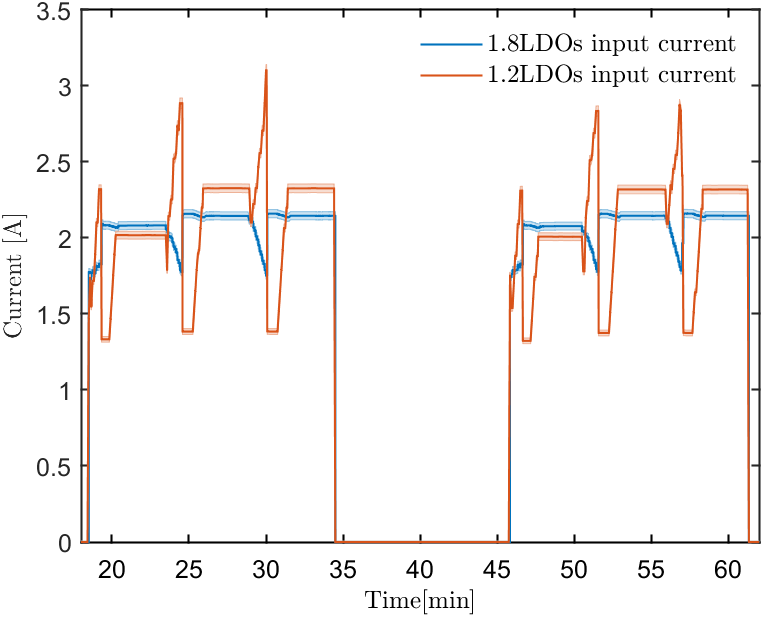
\includegraphics[width=0.6\columnwidth]{Chapter4/images/currents.png}
\caption{Cold startup of one of the \gls{FEB}: current consumed by the 1.8~V and 1.2~V \gls{LDO} regulators during the test procedure. During the period, in which the power is on, each chip undergoes 3 testing cycles.}
\label{fig_power_cycle}
\end{figure}
\newpage
\subsection{Results and onset of failure analysis}
Already during preliminary thermal cycling activities, it was determined that the \gls{LDO}s are more prone to fail than the STS-XYTERs. Therefore, the main effort was put to gain statistics and identify the onset of a potential \gls{LDO} regulator-related failure. To get a better understanding of the conditions leading to failures, the two sets (A and B) of measurements were compared. 


In the case of set B, which featured 8 \glspl{FEB}: 4 \glspl{FEB} with DYMAX 9001, 2 \glspl{FEB} with DYMAX 9008 as the DAM and 9001 as the fill, and 2 \glspl{FEB} without STS-XYTERs and globtop over the \gls{LDO} regulators, during the passive cycling and active cycling no failure was observed. No deterioration was observed under the microscope. First failures were detected during the power cycling at $T=\SI{-30}{\celsius}$, as summarized in the table~\ref{tab:SetA}. 

\begin{table}[!h]
\centering
\caption{Detailed description of the \gls{LDO} failure with regard to the type and number of cycles.}
\resizebox{\textwidth}{!}{%
\begin{tabular}{lll}
Globtop                   & Failure              & Remarks                       \\ \hline
DYMAX Dam 9008, fill 9001 & 100 power cycles     & 1.8V \gls{LDO} failure (AVVD18)      \\ \hline
DYMAX 9001                & 200 power cycles     & 1.2V \gls{LDO} failure after cycling  \\ \hline
DYMAX 9001                & 200/300 power cycles & 1.2V \gls{LDO} failure during cycling \\ \hline
\end{tabular}%
}
\label{tab:SetA}
\end{table}

The onset of the \gls{LDO} failure can be seen in Figure \ref{fig_cold_startup}. At about 500~min the 1.2~V LDO regulators input current started dropping, indicating increasing resistance in the circuit. As depicted in Figure \ref{fig_cold_startup} once the temperature reached $\SI{20}{\celsius}$ the current consumption was again nominal. After about  3000~min, this effect turned out to be irreversible, and we observed the complete failure of the 1.2~V \gls{LDO} regulator. After about 100 cycles, the current consumption measured at the level of the power supply dropped to almost 0~A. 
%\newpage
\begin{figure}[!h]
\centering
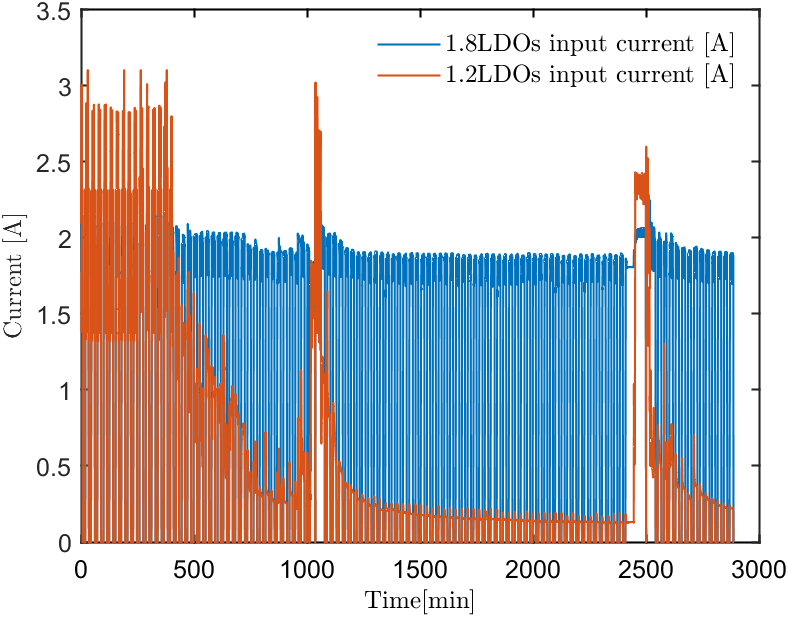
\includegraphics[width=0.46\columnwidth]{Chapter4/images/currents_long.png}
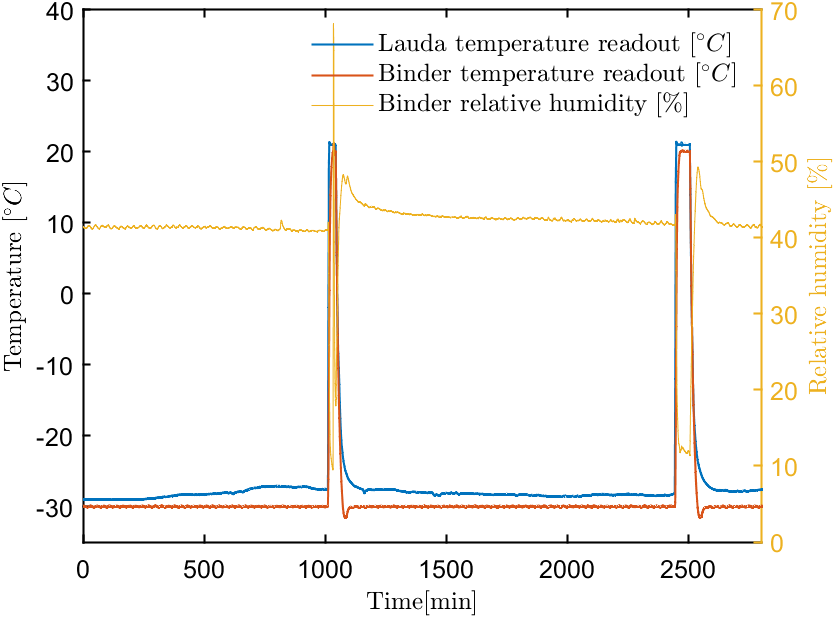
\includegraphics[width=0.48\columnwidth]{Chapter4/images/cycling.png}
\caption{Current consumed by the 1.8V and 1.2 \gls{LDO} regulators during the cold startup testing at $T = \SI{-30}{\celsius}$ (left)
Comparison of the lauda chiller setpoint, readouts from the internal temperature and relative humidity sensors of the climatic chamber (right)}
\label{fig_cold_startup}
\end{figure}

Similarly, the onset of the \gls{FEB} failure can be seen from the diagnostic circuit of the STS-XYTERs (see figure \ref{fig_cold_startup_vddm}). VDDM drops significantly, at the point at which the \gls{LDO} stops providing the nominal current. It was later identified that one of the bond connections from the \gls{LDO} pad failed due to thermal stress. Therefore, the output current of the \gls{LDO} was reduced to a few mA and the supply current to the \glspl{ASIC} was not possible anymore.

\begin{figure}[!h]
\centering
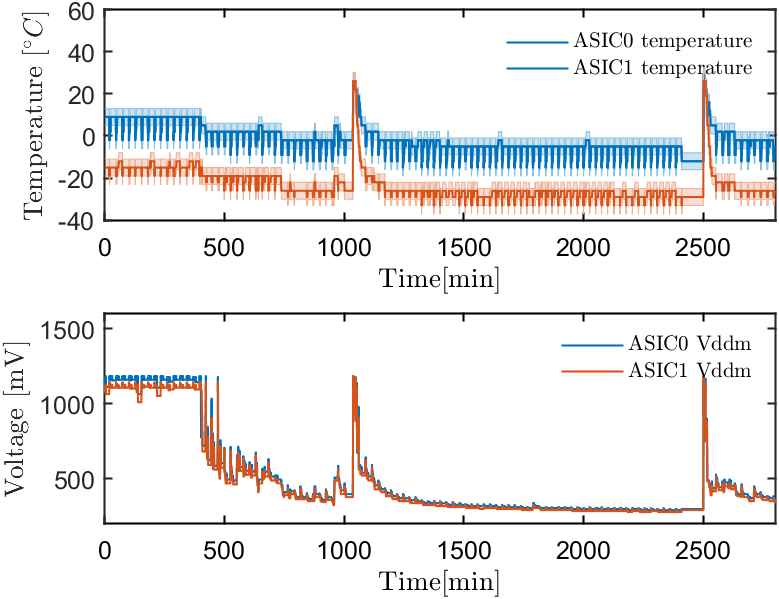
\includegraphics[width=0.6\columnwidth]{Chapter4/images/temps_vddm.png}
\caption{Temperature and VDDM of two chosen STS-XYTERs, and onset of \gls{LDO} regulator failure.}
\label{fig_cold_startup_vddm}
\end{figure}

Similar thermal cycling testing was done to the set A, but in this case, the $\Delta T$ for passive and active cycles was higher, which also lead to an earlier failure of the \gls{PCB} (related to the lift of the \gls{LDO} regulator from the surface of the \gls{PCB}). Exact conditions and moments of failures are summarized in the table \ref{tab:setB}.

\begin{table}[!h]
\centering
\caption{Detailed description of the \gls{LDO} failure with regard to the type and number of cycles}
\resizebox{\textwidth}{!}{%
\begin{tabular}{llll}
Globtop    & Cycles                                                                                                                                                                                                                                                                                  & Failure                                                          & Remarks                                                                              \\ \hline
DYMAX 9001 & \begin{tabular}[c]{@{}l@{}}50 passive cycles {[}$\SI{-20}{\celsius}, \SI{20}{\celsius}${]}\\ 50 active cycles {[}$\SI{-20}{\celsius}, \SI{20}{\celsius}${]}\\ 50 cold startups at $T=\SI{-20}{\celsius}$\end{tabular}                                                                   & 43th active cycle {[}$\SI{-30}{\celsius}, \SI{-20}{\celsius}${]} & 1.2V \gls{LDO} failure                                                                     \\ \hline
DYMAX 9001 & \begin{tabular}[c]{@{}l@{}}50 passive cycles {[}$\SI{-20}{\celsius},\SI{20}{\celsius}${]}\\ 50 active cycles {[}$\SI{-20}{\celsius}, \SI{20}{\celsius}${]}\\ 50 cold startups at $T=\SI{-20}{\celsius}$, \\ 50 active cycles {[}$\SI{-30}{\celsius}, \SI{20}{\celsius}${]}\end{tabular} & 40th cold startup at $T=\SI{-30}{\celsius}$                      & \begin{tabular}[c]{@{}l@{}}failure of both 1.2V \gls{LDO}s\\ 1.8V \gls{LDO} failure\end{tabular} \\ \hline
DYMAX 9001 & \begin{tabular}[c]{@{}l@{}}50 passive cycles {[}$\SI{-30}{\celsius}, \SI{20}{\celsius}${]}\\ 50 active cycles {[}$\SI{-30}{\celsius}, \SI{20}{\celsius}${]}\end{tabular}                                                                                                                & 29th cold startup {$\SI{-40}{\celsius}$}   & 1.2V \gls{LDO} failure                                                                     \\ \hline
\end{tabular}%
}
\label{tab:setB}
\end{table}

The onset of failure during the active cycling can also be seen via the diagnostic circuit of the STS-XYTER (see figure~\ref{fig_active_failure}). The temperature measured by the chip drops by $\SI{15}{\celsius}$, and the VDDM reaches 0~mV, indicating a problem with 1.2~V \gls{LDO} regulator. 

\begin{figure}[!h]
\centering
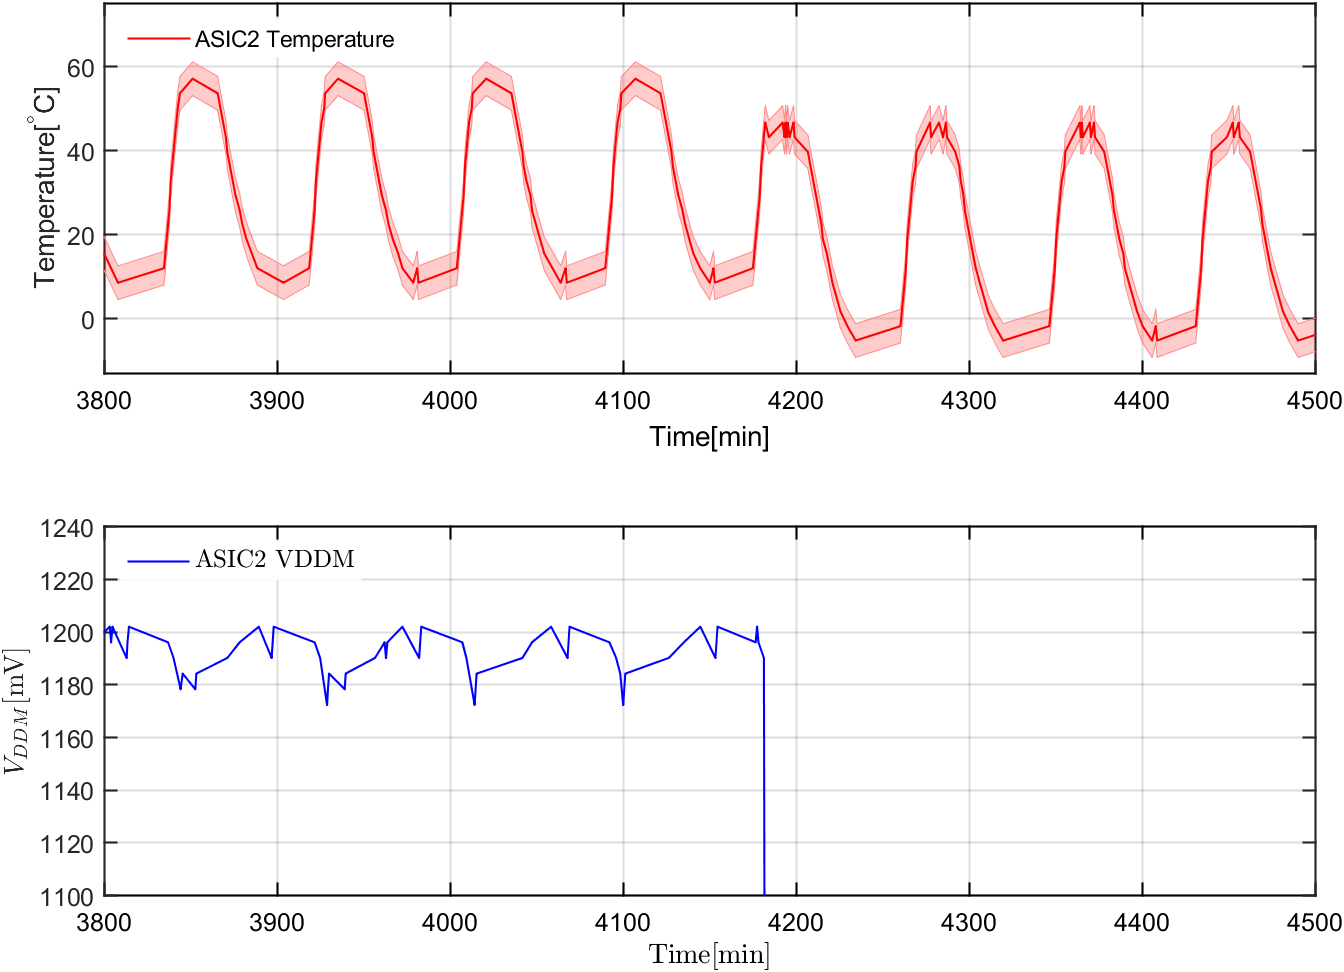
\includegraphics[width=0.6\columnwidth]{Chapter4/images/FEB2ASIC2COMP1.png}
\caption{Temperature and VDDM of a chosen STS-XYTER, and onset of \gls{LDO} regulator failure}
\label{fig_active_failure}
\end{figure}

One of the potential failure mechanisms can be seen in Figure~\ref{fig_ldo_lift}. An air bubble seen on the right photo caused the regulator to lift from the \glspl{PCB} surface. Hence, the \gls{LDO} wasn't providing the nominal voltage and current to the chips. 

\begin{figure}[!h]
\centering
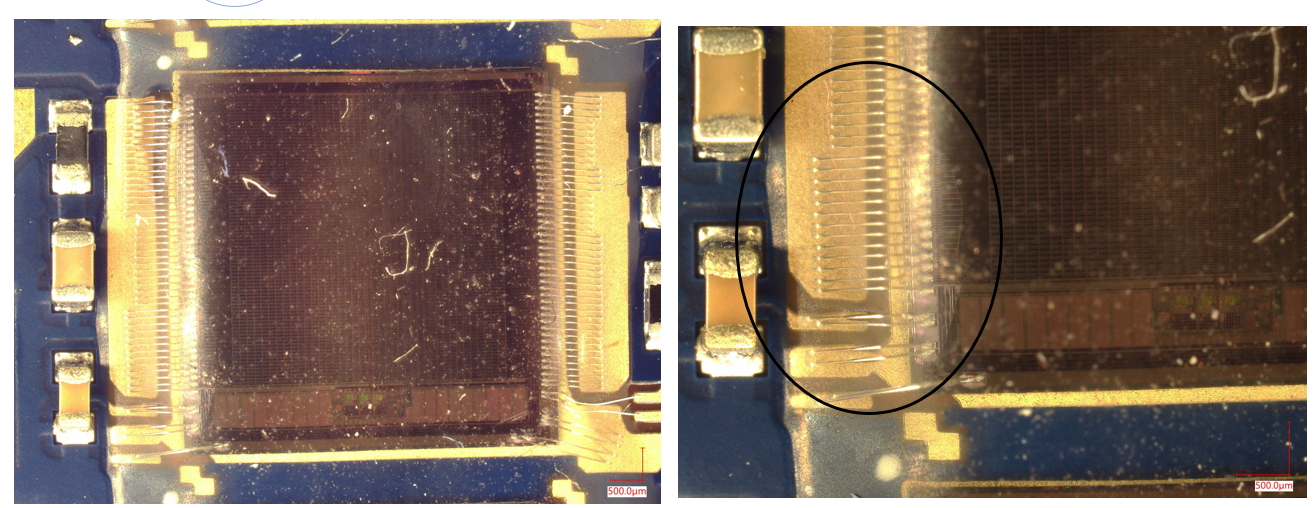
\includegraphics[width=0.8\columnwidth]{Chapter4/images/FEB_81_LDO_lift.png}
\caption{Microscopic view of the air bubble between glob top and bonds of the \gls{LDO}}
\label{fig_ldo_lift}
\end{figure}
\newpage
\subsection{Conclusions}
The deployed setup for the thermal cycling of the \gls{STS} electronics allowed to automate the cycling process, store the necessary date and analyze it in order to better understand the capabilities of the \glspl{FEB}.

Performed thermal cycling lead to discovering the limits of the \glspl{FEB}, namely failures related to the \gls{LDO} regulators. The two realized sets of measurements lead to 6/20 1.2~V \gls{LDO} failures and 2/20 1.8~V \gls{LDO} regulator-related failures. The more frequent 1.2~V \gls{LDO} regulator failure can be associated with larger current changes, leading to larger temperature differences. Furthermore, the boards which were initially tested in harsher conditions (bigger difference between the extreme temperatures) tend to fail sooner.

As described in the introduction to thermal cycling, one of the most probable mechanisms leading to the \gls{LDO} regulator-related failure is the mismatch of the \gls{CTE}. It may potentially result in failure of the \gls{LDO} regulator due to the lift of bonds.

Findings made in this section provide important information on how to improve the module and their performance before the mass production of the modules for the final \gls{STS}. 

%\begin{figure}[!h]
%\centering
%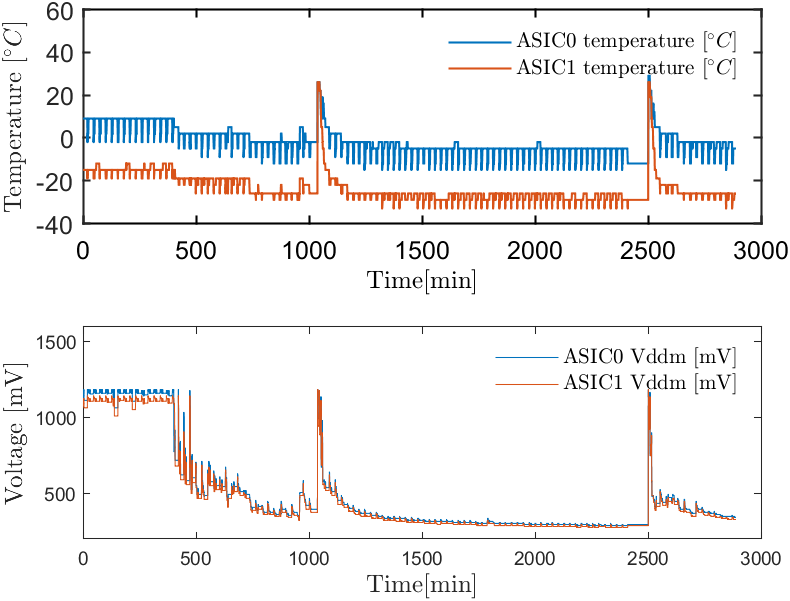
\includegraphics[width=0.6\columnwidth]{Chapter4/images/temps.png}
%\caption{A power cycle}
%\label{fig_cold_startup}
%\end{figure}

%\begin{figure}[!h]
%\centering
%\includegraphics[width=0.6\columnwidth]%{Chapter4/images/csa.png}
%\caption{A power cycle}
%\label{fig_cold_startup}
%\end{figure}

\newpage